\section{Opis implementacije praktičnog rada}

\subsection{Instalacija i konfiguracija okruženja}

\subsubsection{Početni komplet Laravel Jetstream}
Kako bi developerima uštedio vrijeme u samome početku razvijanja nove aplikacije, Laravel nudi autentikacijske i aplikacijske početne komplete (engl.~\textit{starter kits}) kao što su Laravel Breeze i Laravel Jetstream koji automatski pružaju rute, kontrolere i poglede (engl. \textit{views}) potrebne za registraciju i autentikaciju~\cite{starterKits}.

Laravel Jetstream dizajniran je koristeći \textbf{Tailwind CSS}, \textit{utility-first} CSS razvojni okvir. Datoteke \texttt{postcss.config.js} i \texttt{tailwind.config.js} koriste se pri \textit{buildanju} kompajliranog CSS-a aplikacije.

Značajke koje početni komplet Laravel Jetstream pruža su autentikacija, registracija, upravljanje korisničkim profilima, ponovno postavljanje lozinke, verifikacija e-adrese, dvostruka provjera autentičnosti (engl. \textit{two-factor authentication}), upravljanje aktivnim sesijama u web preglednicima, API podrška te opcionalne opcije za upravljanje timovima~\cite{jetstreamIntro}.

Instalira se koristeći Composer, a naredbe za instalaciju prikazane su u ispisu~\ref{jetstreamInstallation}.

\begin{lstlisting}[caption={Naredbe za instalaciju Jetstream paketa u novi Laravel projekt}, label=jetstreamInstallation]
composer create-project laravel/laravel teamstructor-app

cd teamstructor-app

composer require laravel/jetstream
\end{lstlisting}

Jetstream pruža izbor između korištenja \textbf{Livewire} ili Inertia.js \textit{frontend scaffoldinga}. O tom izboru ovisi i odabrani jezik za predloške (engl. \textit{templating language}) jer uz Livewire to je \textbf{Blade}, a uz Inertia.js to je Vue.js~\cite{jetstreamIntro}. \\ Za instaliranje Jetstreama s Livewire \textit{frontend scaffoldingom} i to s uključenom podrškom za timove koristi se naredba \\ \texttt{php artisan jetstream:install livewire -{}-teams}~\cite{jetstreamInstallation}.

\texttt{php artisan vendor:publish -{}-tag=jetstream-views} je naredba čijim se izvršavanjem u \texttt{app} direktoriju kreira direktorij \texttt{resources/view/components} koji sadrži razne generičke Blade komponente čija je svrha da ih se jednostavno može koristiti te pružanje konzistentnog korisničkog sučelja bez potrebe da developer kreira vlastite komponente~\cite{jetstreamLivewire}.

Nakon instalacije Jetstreama potrebno je instalirati i pokrenuti \textit{build} NPM ovisnosti pomoću naredbi \texttt{npm install} i \texttt{npm run build} te migrirati bazu naredbom \texttt{php artisan migrate}~\cite{jetstreamInstallation}.

\subsubsection{\texttt{.env} datoteka}
\texttt{.env} datoteka nalazi se u aplikacijskom root direktoriju i služi kao konfiguracijska datoteka za Laravel web aplikaciju. Pri instalaciji Laravela kreirana je tako da se u nju kopira ogledna konfiguracijska datoteka \texttt{.env.example}~\cite{configuration}. 

Dobra je praksa i zbog sigurnosti i zbog toga što je konfiguracija promjenjiva ovisno o pojedinačnim okruženjima da neenkriptirana \texttt{.env} datoteka nije dio kontrole izvornog k\^oda aplikacije, dok je to u redu za \texttt{.env.example} datoteku te ista može poslužiti kao ogledni primjer s \textit{placeholder} vrijednostima za varijable koje je potrebno definirati~\cite{configuration}.

Primjer definicije varijable može se vidjeti u ispisu~\ref{envDefinition}.

\begin{lstlisting}[caption={Definicija varijable u \texttt{.env} datoteci}, label=envDefinition]
APP_NAME=Teamstructor
\end{lstlisting}

U Laravel aplikaciji pristup vrijednosti pojedine varijable iz \texttt{.env} datoteke moguć je pomoću \texttt{\$\_ENV} PHP superglobalne varijable ili koristeći funkciju \texttt{env}, kao u ispisu~\ref{envRetrieve}.

\begin{lstlisting}[caption={Pristup vrijednosti \textit{environment} varijable u Laravelu}, label=envRetrieve]
'name' => env('APP_NAME', 'Laravel'),
\end{lstlisting}

\subsection{Struktura Laravel aplikacije}

\subsubsection{Struktura početnog direktorija s izvornim k\^odom aplikacije}
Osnovna struktura \textit{root} direktorija Laravel aplikacije jest sljedeća~\cite{structure}:  \\
\dirtree{%
.1 teamstructor-app.
.2 app.
.2 bootstrap.
.2 config.
.2 database.
.2 node\_modules.
.2 public.
.2 resources.
.2 routes.
.2 storage.
.2 tests.
.2 vendor.
}

\begin{itemize}
\item \texttt{app} - Sadrži "jezgru" aplikacije te će biti posebno predstavljen u poglavlju~\ref{subsubsection:app}.
\item \texttt{bootstrap} - Sadrži datoteku \texttt{app.php} koja pokreće razvojni okvir te direktorij \texttt{cache} koji sadrži datoteke predmemorije za optimizaciju performansi.
\item \texttt{config} - Sadrži konfiguracijske datoteke.
\item \texttt{database} - Sadrži migracije, tvornice modela (engl. \textit{model factories}) i \textit{seed}-ove.
\item \texttt{node\_modules} - Nije u osnovnoj strukturi, međutim nastaje instalacijom NPM ovisnosti te sadrži instalirane module tj. biblioteke potrebne za \textit{frontend} dio aplikacije kao poddirektorije.
\item \texttt{public} - Sadrži datoteku \texttt{index.php} koja je polazna točka svih zahtjeva prema aplikaciji te konfigurira automatsko učitavanje (engl. \textit{autoloading}).  Također se tu nalaze i javna "imovina" aplikacije (engl. \textit{assets}): slike te JavaScript i CSS datoteke.
\item \texttt{resources} - Sadrži poglede (engl. \textit{views}) i nekompajlirane JavaScript i CSS datoteke koje su \textit{assets} aplikacije.
\item \texttt{routes} - Sadrži definicije svih ruta u aplikaciji. Zadano su uključene datoteke: \texttt{web.php}, \texttt{api.php}, \texttt{console.php} i \texttt{channels.php}.
\item \texttt{storage} - Služi kao lokalno spremište podataka aplikacije te je podijeljen na direktorije \texttt{app}, \texttt{framework} i \texttt{logs}. Sadrži \texttt{.log} datoteke zapisnika, kompajlirane Blade predloške, sesije, predmemorije datoteka itd.
\item \texttt{tests} - Sadrži skripte za automatizirane aplikacijske testove te dolazi s po jednim oglednim primjerom \textit{unit} i \textit{feature} testova.
\item \texttt{vendor} - Sadrži preuzete Composer ovisnosti aplikacije.
\end{itemize}

\subsubsection{Struktura \texttt{app} direktorija}
\label{subsubsection:app}
Na slici~\ref{fig:appDir} prikazan je sadržaj \texttt{app} direktorija.
\begin{figure}[H]
	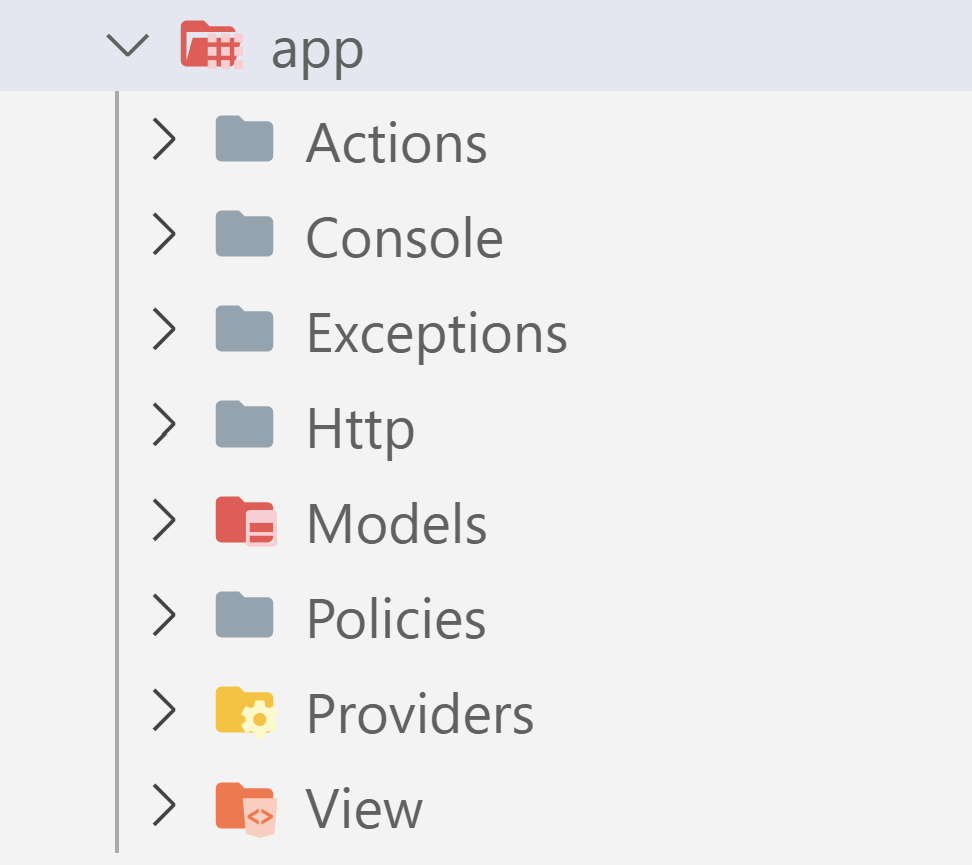
\includegraphics[width=0.4\linewidth,clip=]{assets/app-directory.png}
	\centering
	\caption{Sadržaj \texttt{app} direktorija}
	\label{fig:appDir}
\end{figure}

Možemo vidjeti da se \texttt{app} direktorij sastoji od sljedećih poddirektorija~\cite{structure}: 
\begin{itemize}
\item \texttt{Actions} - Direktorij koji se kreira pri Jetstream instalaciji, a sadrži \texttt{Action} klase koje obično izvode samo jednu akciju i odgovaraju jednoj Jetstream ili Fortify značajki kao npr. kreiranje korisnika ili tima,  postavljanje nove lozinke, brisanje korisnika ili tima, dodavanje člana u tim itd.~\cite{jetstreamActions}
\item \texttt{Console} - Sadrži datoteku \texttt{Kernel.php} u kojoj se registriraju \textit{custom} Artisan naredbe.
\item \texttt{Exceptions} - Sadrži datoteku \texttt{Handler.php} koja upravlja svim iznimkama u aplikaciji te je moguće registrirati nove \textit{custom} iznimke.
\item \texttt{Http} - Gotovo sva logika aplikacije smještena je u ovaj direktorij. Sadrži kontrolere, klase Livewire komponenti te \textit{middleware}.
\item \texttt{Models} - Sadrži klase svih Eloquent modela ove web aplikacije.
\item \texttt{Policies} - Nastaje izvođenjem \texttt{make:policy} Artisan naredbe te sadrži klase u kojima su definirana pravila autorizacije unutar aplikacije.
\item \texttt{Providers} - Sadrži sve davatelje usluga (engl. \textit{service providers}) aplikacije.
\item \texttt{View} - Direktorij se kreira pri Jetstream instalaciji, a sadrži klase Livewire \textit{layout} komponenti - "application" \textit{layout} te "guest" \textit{layout}~\cite{jetstreamLayouts}.
\end{itemize}

Još nekolicina direktorija može biti generirana unutar \texttt{app} direktorija izvršavanjem Artisan \texttt{make} naredbi za generiranje klasa~\cite{structure}. 

\subsection{Struktura relacijske baze podataka}
Na slici~\ref{fig:erDiagram} prikazan je ER (engl. \textit{Entity Relationship}) dijagram relacijske baze podataka u phpMyAdmin sučelju na kojemu možemo vidjeti tablice u koje su podatci spremani te njihove međusobne relacije.
\begin{figure}[H]
	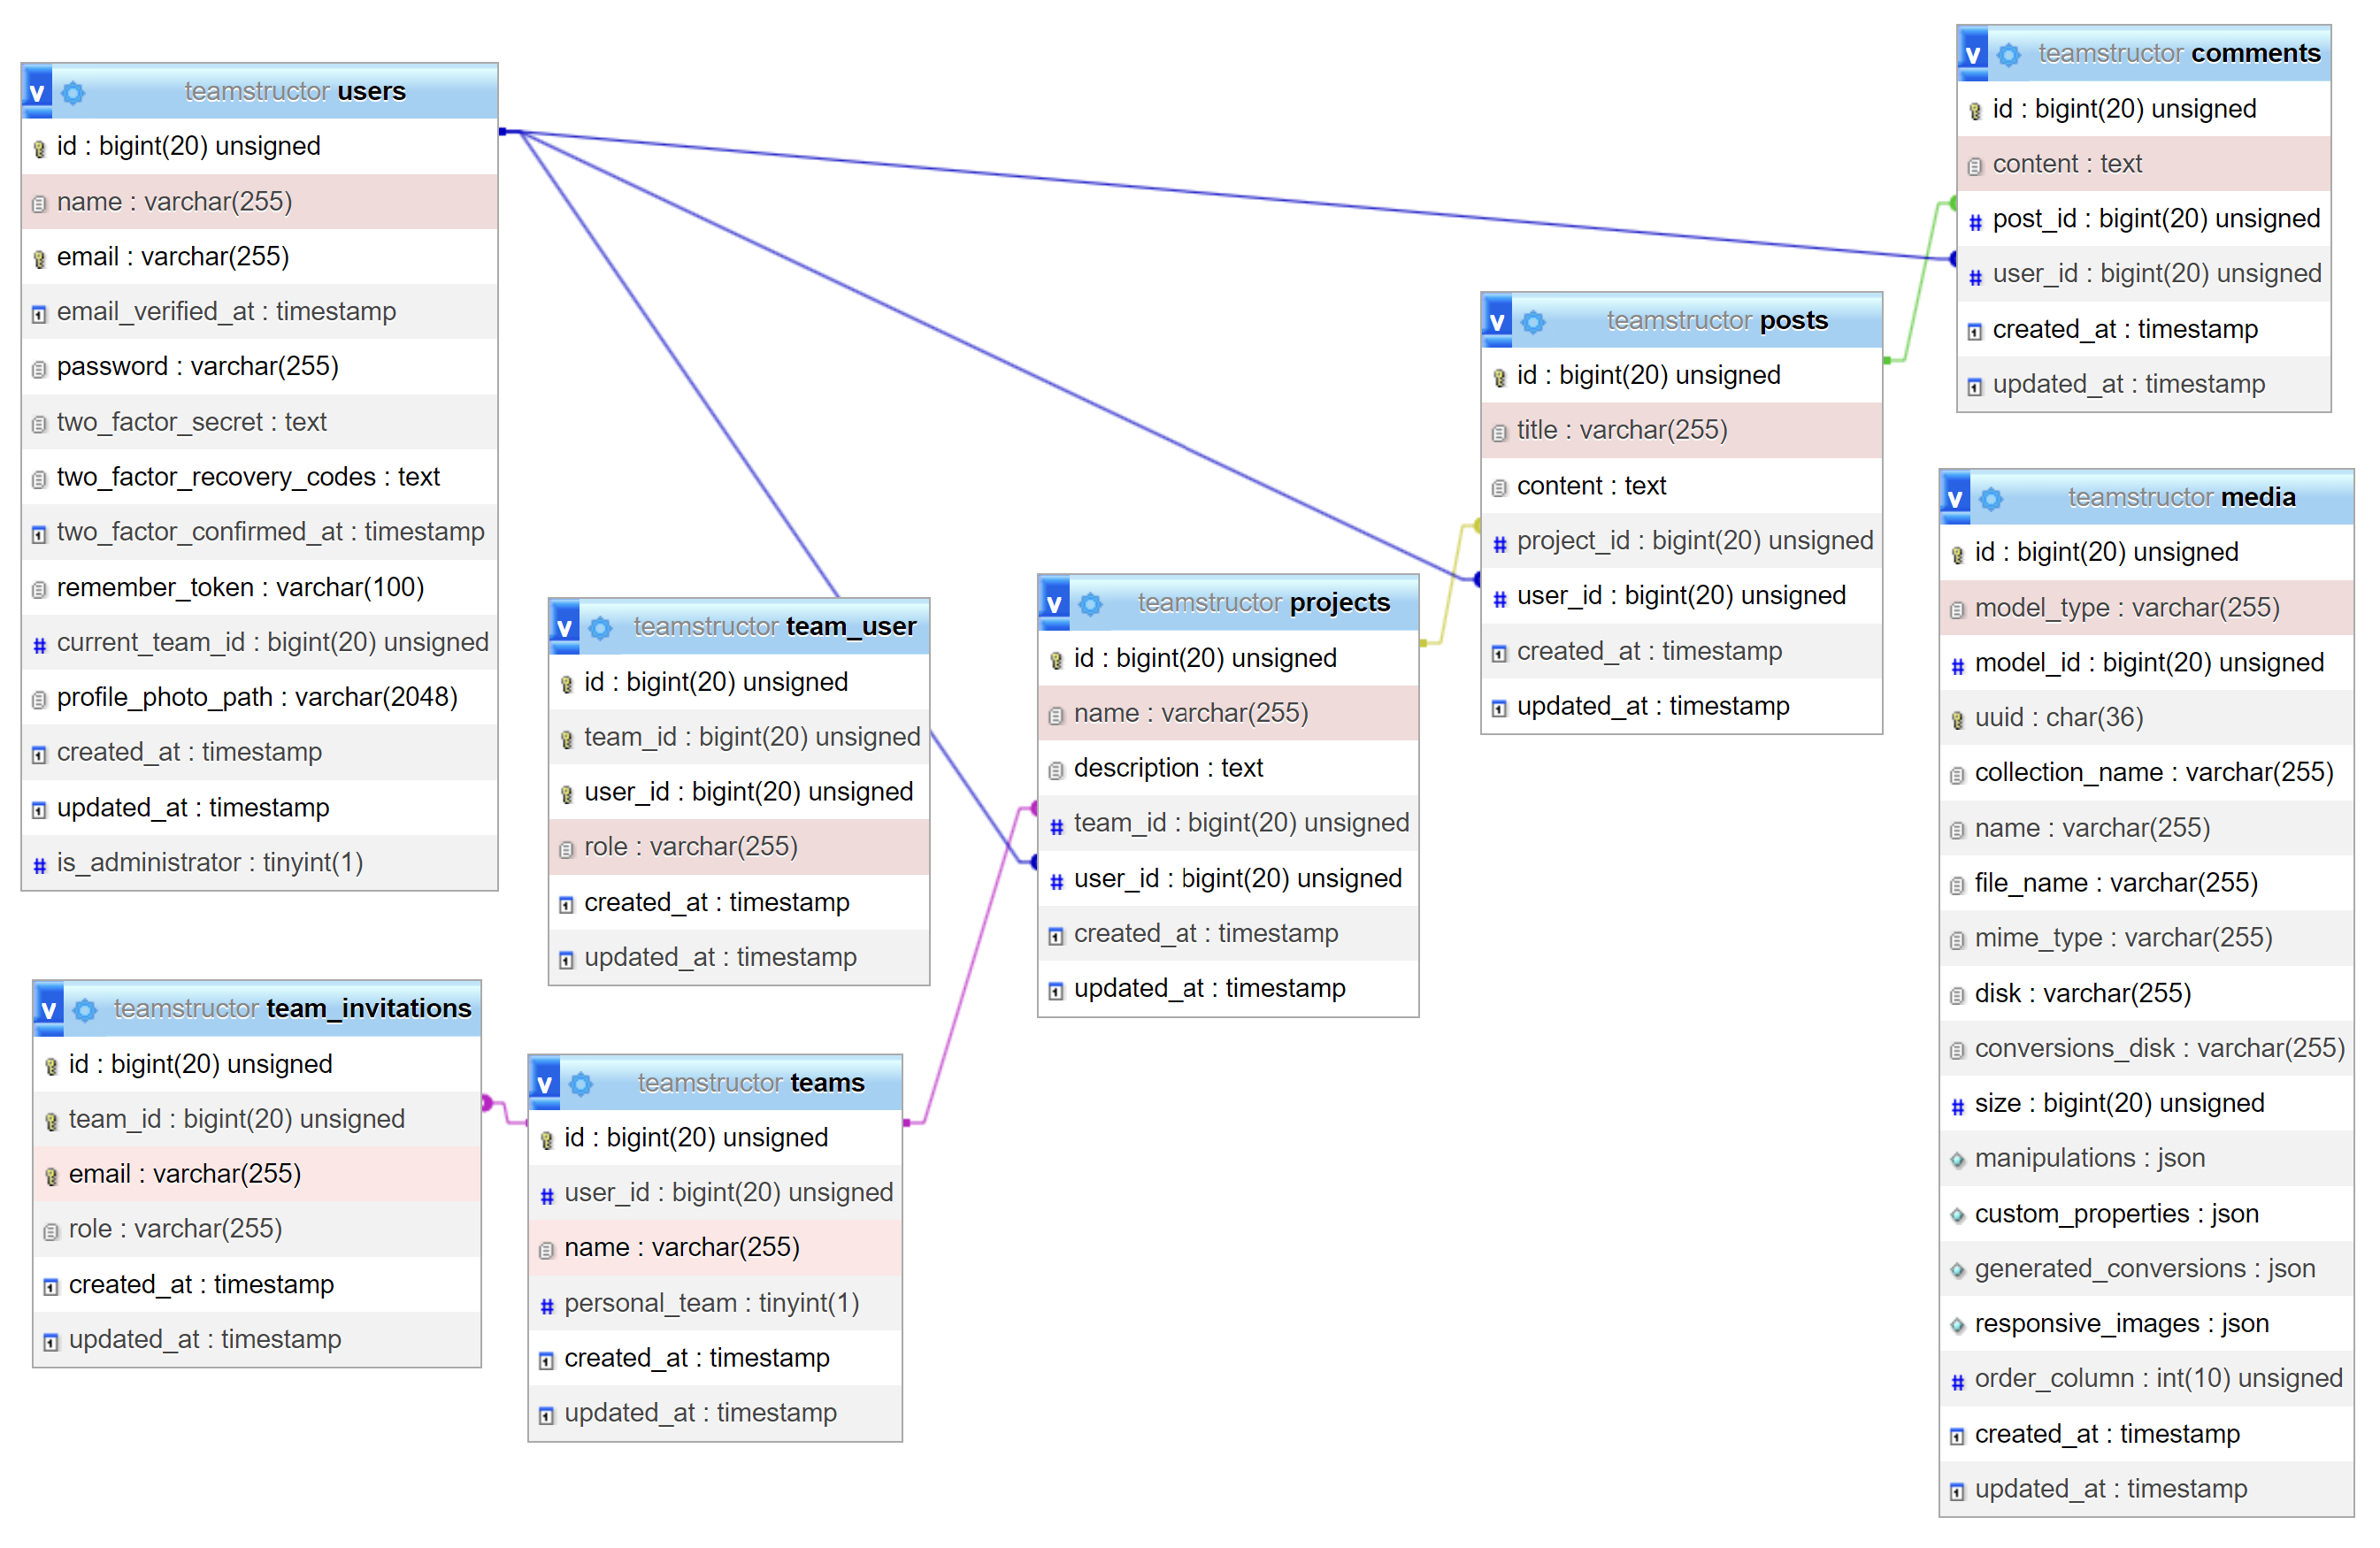
\includegraphics[width=1\linewidth,clip=]{assets/db-er-diagram.png}
	\centering
	\caption{Dijagram relacijske baze podataka}
	\label{fig:erDiagram}
\end{figure}

Radi preglednosti su na dijagramu sa slike~\ref{fig:erDiagram} prikazane samo tablice koje se odnose na modele, a izostavljene su tablice: 
\begin{itemize}
\item \texttt{failed\_jobs} - Automatski prisutna u Laravel aplikacijama, služi za pohranu poslova iz reda čekanja koji se nisu uspjeli izvršiti.
\item \texttt{migrations} - Automatski prisutna u Laravel aplikacijama, služi za pohranu migracija.
\item \texttt{password\_reset\_tokens} - Automatski prisutna u Laravel aplikacijama, služi za pohranu tokena za ponovno postavljanje lozinki u aplikaciji.
\item \texttt{personal\_access\_tokens} - Kreira ju Laravel Sanctum pri instalaciji Laravel Jetstreama, a služi za pohranu API tokena u aplikaciji.
\item \texttt{sessions} - Kada se koristi \texttt{database} \textit{driver} za sesije, onda se u ovu tablicu iste pohranjuju.
\item \texttt{telescope\_entries}, \texttt{telescope\_entries\_tags}, \\ \texttt{telescope\_monitoring} - Nastaju pri instalaciji Laravel Telescopea, a služe za pohranu podataka za Telescope.
\end{itemize}

U poglavlju~\ref{subsection:dbInteraction} će biti više rečeno o načinima na koje se ostvaruje interakcija s bazom podataka te o samim modelima i relacijama.

\subsection{Interakcija s bazom podataka}
\label{subsection:dbInteraction}

\subsubsection{Migracije}
Migracije služe kao kontrola verzije baze podataka. U Laravelu migracije koriste fasadu (engl. \textit{facade}) \texttt{Schema} koja pruža \textit{database agnostic} podršku za sve sustave baza podataka koje Laravel podržava~\cite{migrations}.

Migracija se može kreirati pozivom \texttt{make:migration} Artisan naredbe te će se ista smjestiti u \texttt{database/migrations} direktorij. Nazivu svake migracije dodaje se pripadajući \textit{timestamp} prema kojem Laravel prati redoslijed migracija~\cite{migrations}.

Sama migracijska klasa sadrži dvije metode: \texttt{up} koja kreira ili modificira tablice, stupce ili indekse u bazi podataka te \texttt{down} koja bi trebala poništiti promjene učinjene u \texttt{up} metodi inverznim operacijama~\cite{migrations}.

U ispisu~\ref{projectsTableMigration} možemo vidjeti k\^od migracije za kreiranje tablice \texttt{projects} u kojoj u \texttt{up} metodi kreiramo tablicu navodeći njezin naziv i stupce koje sadrži, a u \texttt{down} metodi poništavamo operacije izvedene u \texttt{up} metodi na način da se odbacuje novokreirana tablica tj. izvodi \textit{drop} tablice.

\begin{lstlisting}[caption={Migracija za kreiranje tablice \texttt{projects}}, label=projectsTableMigration]
<?php

use Illuminate\Database\Migrations\Migration;
use Illuminate\Database\Schema\Blueprint;
use Illuminate\Support\Facades\Schema;

return new class extends Migration
{
    /**
     * Run the migrations.
     */
    public function up(): void
    {
        Schema::create('projects', function (Blueprint $table) {
            $table->id();
            $table->string('name');
            $table->text('description');
            $table->foreignId('team_id')->constrained();
            $table->foreignId('user_id')->constrained();
            $table->timestamps();
        });
    }

    /**
     * Reverse the migrations.
     */
    public function down(): void
    {
        Schema::dropIfExists('projects');
    }
};

\end{lstlisting}

U ispisu~\ref{administratorColumnMigration} prikazana je migracija koja modificira tablicu \texttt{users} tako da joj dodaje stupac \texttt{is\_administrator}. U \texttt{up} metodi definira se stupac koji će se dodati, a u \texttt{down} metodi te promjene će biti poništene odbacivanjem novododanog stupca metodom \texttt{dropColumn}.

\begin{lstlisting}[caption={Migracija za dodavanje stupca \texttt{is\_administrator} u tablicu \texttt{users}}, label=administratorColumnMigration]
<?php

use Illuminate\Database\Migrations\Migration;
use Illuminate\Database\Schema\Blueprint;
use Illuminate\Support\Facades\Schema;

return new class extends Migration
{
    /**
     * Run the migrations.
     */
    public function up(): void
    {
        Schema::table('users', function (Blueprint $table) {
            $table->boolean('is_administrator')->default(false);
        });
    }

    /**
     * Reverse the migrations.
     */
    public function down(): void
    {
        Schema::table('users', function (Blueprint $table) {
            $table->dropColumn('is_administrator');
        });
    }
};

\end{lstlisting}

Za izvršiti sve migracije koje se još nisu primjenile na bazu podataka pokreće se Artisan naredba \texttt{migrate}, a za povratak na prethodnu migraciju tj. poništavanje promjena posljednjih \textit{n} migracija Artisan naredba \texttt{migrate:rollback}~\cite{migrations}.

\subsubsection{Populacija podatcima}
Populacija baze podataka (engl. \textit{seeding}) u Laravelu se može obaviti koristeći \textit{seed} klase koje se nalaze u direktoriju \texttt{database/seeders}. Ondje se zadano nalazi \\ \texttt{DatabaseSeeder} klasa koja sadrži metodu \texttt{run} koja se izvršava pozivom \texttt{db:seed} Artisan naredbe. Unutar metode \texttt{run} koristeći se metodom \texttt{call} pozivaju se dodatni ostali u aplikaciji definirani \textit{seederi}. Dobra je praksa \textit{seeding} k\^od podijeliti u više dijelova tj. \textit{seed} klasa jer se tako ne "zatrpava" isključivo jedan \textit{seeder} k\^odom. U ispisu~\ref{databaseSeeder} može se vidjeti \textit{seedere} pozvane koristeći metodu \texttt{call}~\cite{seeding}.

\begin{lstlisting}[caption={Sadržaj \texttt{DatabaseSeeder} klase}, label=databaseSeeder]
<?php

namespace Database\Seeders;

// use Illuminate\Database\Console\Seeds\WithoutModelEvents;
use Illuminate\Database\Seeder;

class DatabaseSeeder extends Seeder
{
    /**
     * Seed the application's database.
     */
    public function run(): void
    {
        $this->call([
            UserSeeder::class,
            TeamSeeder::class,
            ProjectSeeder::class,
            PostSeeder::class,
            CommentSeeder::class,
            ResourceSeeder::class,
        ]);
    }
}

\end{lstlisting}

Samo ubacivanje podataka u bazu podataka koristeći \textit{seedere} može se ostvariti ručno koristeći \textit{query builder} ili koristeći Eloquent tvornice modela (engl. \textit{model factories}) o čemu će biti više riječi u nastavku.

\subsubsection{Eloquent ORM}
Eloquent ORM (engl. \textit{object-relational mapper}) je Laravelova biblioteka za objektno-relacijsko mapiranje čija je uloga olakšati interakcije s bazom podataka jer obavlja konverziju k\^oda napisanog u objektno orijentiranom jeziku u jezik relacijske baze podataka i obrnuto. Omogućava stvaranje virtualne objektne baze podataka koja je prilagođena korištenju unutar programskog jezika~\cite{eloquent}.

\paragraph{Modeli i tvornice modela}\mbox{}\\
\indent Eloquent modeli nalaze se u direktoriju \texttt{app/Models} te se za stvaranje novog modela koristi Artisan naredba \texttt{make:model}. Svaka tablica baze podataka odgovara jednom Eloquent modelu te će on biti korišten za operacije nad istom. Prema konvenciji, ako drugačije nije definirano u samoj klasi, naziv odgovarajuće tablice je naziv klase modela u množini u \textit{snake caseu}. Tako su u tablici~\ref{fig:namingModelTable} prikazani nazivi klasa modela te odgovarajući nazivi tablica (koje su prikazane i na slici~\ref{fig:erDiagram}).

\begin{longtable}{ll}
\caption{Nazivi klasa modela i pripadajuće tablice}\label{fig:namingModelTable}
\endfirsthead
\endhead
\hline
Naziv klase modela&Naziv odgovarajuće tablice\\
\hline
\lstinline!Comment!&comments\\
\lstinline!Membership!&team\_user\\
\lstinline!Post!&posts\\
\lstinline!Project!&projects\\
\lstinline!Resource!&media\\
\lstinline!Team!&teams\\
\lstinline!TeamInvitation!&team\_invitations\\
\lstinline!User!&users\\
\hline
\end{longtable}

U klasi modela definiramo njegove atribute (\textit{fillable} - one koji su \textit{mass assignable} tj. dozvoljeno je da ih dodijele korisnici aplikacije te \textit{hidden} - one koji su skriveni pri serijalizaciji), relacije (o kojima će biti više riječi u poglavlju~\ref{paragraph:relations}), \textit{traits} tj. osobine koje koristi, događaje koje šalje itd.

U ispisu~\ref{modelUser} prikazan je dio k\^oda iz klase modela \texttt{User} gdje je vidljivo da koristi nekolicinu osobina (engl. \textit{traits}) te definiranje atributa modela.

\begin{lstlisting}[caption={Dio k\^oda model klase \texttt{User}}, label=modelUser]
<?php

namespace App\Models;

use Illuminate\Database\Eloquent\Factories\HasFactory;
use Illuminate\Database\Eloquent\Relations\HasMany;
use Illuminate\Foundation\Auth\User as Authenticatable;
use Illuminate\Notifications\Notifiable;
use Laravel\Fortify\TwoFactorAuthenticatable;
use Laravel\Jetstream\HasProfilePhoto;
use Laravel\Jetstream\HasTeams;
use Laravel\Sanctum\HasApiTokens;

class User extends Authenticatable
{
    use HasApiTokens;
    use HasFactory;
    use HasProfilePhoto;
    use HasTeams;
    use Notifiable;
    use TwoFactorAuthenticatable;

    /**
     * The attributes that are mass assignable.
     *
     * @var array<int, string>
     */
    protected $fillable = [
        'name', 'email', 'password',
    ];

    /**
     * The attributes that should be hidden for serialization.
     *
     * @var array<int, string>
     */
    protected $hidden = [
        'password',
        'remember_token',
        'two_factor_recovery_codes',
        'two_factor_secret',
        'is_administrator',
    ];

    /**
     * The attributes that should be cast.
     *
     * @var array<string, string>
     */
    protected $casts = [
        'email_verified_at' => 'datetime',
    ];

    /**
     * The accessors to append to the model's array form.
     *
     * @var array<int, string>
     */
    protected $appends = [
        'profile_photo_url',
    ];
    
// ...
\end{lstlisting}

U ispisu~\ref{modelUser} možemo primjetiti da model \texttt{User} koristi osobinu \texttt{HasFactory}. Pomoću tvornica modela (engl. \textit{model factories}) može se definirati skup zadanih atributa za određeni Eloquent model pa je olakšano populiranje baze podataka sa testnim zapisima. Tvornica modela može se generirati Artisan naredbom \texttt{make:factory} te će se nalaziti u \texttt{database/factories} direktoriju~\cite{factories}.

U ispisu~\ref{factoryUser} prikazan je dio k\^oda iz tvornice modela \texttt{UserFactory} gdje je vidljiva metoda \texttt{definition} koja vraća skup atributa koji bi se trebali primijeniti na model pri njegovom kreiranju. Za generiranje testnih lažnih podataka koristi se Faker~\cite{fakerGitHub} PHP biblioteka čija je instanca u \texttt{\$this->faker}~\cite{factories}.

\begin{lstlisting}[caption={Dio k\^oda tvornice modela \texttt{UserFactory}}, label=factoryUser]
<?php

namespace Database\Factories;

use App\Models\Team;
use App\Models\User;
use Illuminate\Database\Eloquent\Factories\Factory;
use Illuminate\Support\Str;
use Laravel\Jetstream\Features;

class UserFactory extends Factory
{
    /**
     * The name of the factory's corresponding model.
     *
     * @var string
     */
    protected $model = User::class;

    /**
     * Define the model's default state.
     *
     * @return array<string, mixed>
     */
    public function definition(): array
    {
        return [
            'name' => $this->faker->name(),
            'email' => $this->faker->unique()->safeEmail(),
            'email_verified_at' => now(),
            'password' => '...', // password
            'two_factor_secret' => null,
            'two_factor_recovery_codes' => null,
            'remember_token' => Str::random(10),
            'profile_photo_path' => null,
            'current_team_id' => null,
            'is_administrator' => false,
        ];
    }
    
// ...
\end{lstlisting}

Također, tvornicama modela možemo definirati stanja (engl. \textit{factory states}) koja predstavljaju način da se primijene diskretne izmjene tj. modificiraju atributi na nekoj tvornici modela. U ispisu~\ref{factoryStatesUser} prikazan je dio k\^oda iz tvornice modela \texttt{UserFactory} gdje se definira stanje tvornice modela za stvaranje administrator korisnika. Vidljivo je da to stanje vrši izmjene samo na odabranim atributima, a ostali atributi će biti postavljeni kao u izvornoj definiciji tvornice modela~\cite{factories}.

\begin{lstlisting}[caption={Dio k\^oda tvornice modela \texttt{UserFactory} koji prikazuje definiciju stanja tvornice modela}, label=factoryStatesUser]
    /**
     * Indicate that the user is administrator.
     */
    public function administrator(): static
    {
        return $this->state(function (array $attributes) {
            return [
                'name' => 'Admin Admin',
                'email' => 'admin@teamstructor.test',
                'is_administrator' => true,
            ];
        });
    }
\end{lstlisting}

\paragraph{Relacije}
\label{paragraph:relations}\mbox{}\\
\indent Odnosi tj. relacije između modela definiraju se unutar samih klasa Eloquent modela kao metode. Možemo ponovno pogledati sliku~\ref{fig:erDiagram} i obratiti pozornost na veze među modelima.

Model \texttt{User} definira veze prema modelima \texttt{Project}, \texttt{Post} i \texttt{Comments} kao što je vidljivo u ispisu~\ref{relationsUser}, a u osobini \texttt{HasTeams} koju model koristi definirane su veze prema modelima \texttt{Team} i \texttt{Membership} te su te metode prikazane u ispisu~\ref{relationsUserTrait}.

\begin{lstlisting}[caption={Relacije modela \texttt{User}}, label=relationsUser]
    /**
     * Get the projects created by user.
     */
    public function projects(): HasMany
    {
        return $this->hasMany(Project::class);
    }

    /**
     * Get the user's posts.
     */
    public function posts(): HasMany
    {
        return $this->hasMany(Post::class);
    }

    /**
     * Get the user's comments.
     */
    public function comments(): HasMany
    {
        return $this->hasMany(Comment::class);
    }
\end{lstlisting}

\begin{lstlisting}[caption={Relacije modela \texttt{User} koje koristi iz osobine \texttt{HasTeams}}, label=relationsUserTrait]
    /**
     * Get all of the teams the user owns.
     *
     * @return \Illuminate\Database\Eloquent\Relations\HasMany
     */
    public function ownedTeams()
    {
        return $this->hasMany(Jetstream::teamModel());
    }

    /**
     * Get all of the teams the user belongs to.
     *
     * @return \Illuminate\Database\Eloquent\Relations\BelongsToMany
     */
    public function teams()
    {
        return $this->belongsToMany(
                        Jetstream::teamModel(), 
                        Jetstream::membershipModel()
                    )->withPivot('role')
                    ->withTimestamps()
                    ->as('membership');
    }
\end{lstlisting}

Model \texttt{Team} definira veze prema modelu \texttt{Project}, kao što je vidljivo u ispisu~\ref{relationsTeam}, a nasljeđujući model \texttt{JetstreamTeam} definirane su veze prema modelima \texttt{User}, \\ \texttt{Membership} i \texttt{TeamInvitation} te su te metode prikazane u ispisu~\ref{relationsJetstreamTeam}.

\begin{lstlisting}[caption={Relacije modela \texttt{Team}}, label=relationsTeam]
<?php

namespace App\Models;

// ...
use Illuminate\Database\Eloquent\Relations\HasMany;
// ...
use Laravel\Jetstream\Team as JetstreamTeam;

class Team extends JetstreamTeam
{

// ...

    /**
     * Get the projects for the team.
     */
    public function projects(): HasMany
    {
        return $this->hasMany(Project::class)->latest();
    }
    
// ...
\end{lstlisting}

\begin{lstlisting}[caption={Relacije modela \texttt{Team} koje nasljeđuje od modela \texttt{JetstreamTeam}}, label=relationsJetstreamTeam]
    /**
     * Get the owner of the team.
     *
     * @return \Illuminate\Database\Eloquent\Relations\BelongsTo
     */
    public function owner()
    {
        return $this->belongsTo(Jetstream::userModel(), 'user_id');
    }
    
    /**
     * Get all of the users that belong to the team.
     *
     * @return \Illuminate\Database\Eloquent\Relations\BelongsToMany
     */
    public function users()
    {
        return $this->belongsToMany(
                    Jetstream::userModel(), 
                    Jetstream::membershipModel()
                )->withPivot('role')
                ->withTimestamps()
                ->as('membership');
    }
    
    /**
     * Get all of the pending user invitations for the team.
     *
     * @return \Illuminate\Database\Eloquent\Relations\HasMany
     */
    public function teamInvitations()
    {
        return $this->hasMany(Jetstream::teamInvitationModel());
    }
\end{lstlisting}

Model \texttt{Membership} je pivotni model (između modela \texttt{Team} i \texttt{User}), a model \\ \texttt{TeamInvitation} definira vezu prema modelu \texttt{Team} kao što je prikazano u ispisu~\ref{relationsTeamInvitation}:

\begin{lstlisting}[caption={Relacije modela \texttt{TeamInvitation}}, label=relationsTeamInvitation]
    /**
     * Get the team that the invitation belongs to.
     */
    public function team(): BelongsTo
    {
        return $this->belongsTo(Jetstream::teamModel());
    }
\end{lstlisting}

Model \texttt{Project} definira veze prema modelima \texttt{Team}, \texttt{User} i \texttt{Post} vidljivo u ispisu~\ref{relationsProject}, te implementirajući \textit{interface} \texttt{HasMedia} i koristeći osobinu \\ \texttt{InteractsWithMedia} definira i vezu prema modelu \texttt{Resource} vidljivo u ispisu~\ref{relationsProjectTrait}.

\begin{lstlisting}[caption={Relacije modela \texttt{Project}}, label=relationsProject]
<?php

namespace App\Models;

// ...
use Illuminate\Database\Eloquent\Model;
use Illuminate\Database\Eloquent\Relations\BelongsTo;
use Illuminate\Database\Eloquent\Relations\HasMany;
use Spatie\MediaLibrary\HasMedia;
use Spatie\MediaLibrary\InteractsWithMedia;

class Project extends Model implements HasMedia
{
    // ...
    use InteractsWithMedia;
    
    // ...
    
    /**
     * Get the team that owns the project.
     */
    public function team(): BelongsTo
    {
        return $this->belongsTo(Team::class);
    }

    /**
     * Get the user that created the project.
     */
    public function user(): BelongsTo
    {
        return $this->belongsTo(User::class);
    }

    /**
     * Get the posts for the project.
     */
    public function posts(): HasMany
    {
        return $this->hasMany(Post::class)
                    ->with(['user', 'comments'])
                    ->latest();
    }
    
// ...
\end{lstlisting}

\begin{lstlisting}[caption={Relacije modela \texttt{Project} koje koristi iz osobine \texttt{InteractsWithMedia}}, label=relationsProjectTrait]
public function media(): MorphMany
{
    return $this->morphMany(config('media-library.media_model'), 'model');
}
\end{lstlisting}

Model \texttt{Post} definira veze prema modelima \texttt{Project}, \texttt{User} i \texttt{Comment} kao što je prikazano u ispisu~\ref{relationsPost}, a model \texttt{Comment} definira veze prema modelima \texttt{Post} i \texttt{User}, prikazano u ispisu~\ref{relationsComment}.

\begin{lstlisting}[caption={Relacije modela \texttt{Post}}, label=relationsPost]
    /**
     * Get the project that owns the post.
     */
    public function project(): BelongsTo
    {
        return $this->belongsTo(Project::class);
    }

    /**
     * Get the author of the post.
     */
    public function user(): BelongsTo
    {
        return $this->belongsTo(User::class);
    }

    /**
     * Get the comments for the post.
     */
    public function comments(): HasMany
    {
        return $this->hasMany(Comment::class)->latest();
    }
\end{lstlisting}

\begin{lstlisting}[caption={Relacije modela \texttt{Comment}}, label=relationsComment]
    /**
     * Get the post that owns the comment.
     */
    public function post(): BelongsTo
    {
        return $this->belongsTo(Post::class);
    }

    /**
     * Get the author of the comment.
     */
    public function user(): BelongsTo
    {
        return $this->belongsTo(User::class);
    }
\end{lstlisting}

Model \texttt{Resource} nasljeđujući model \texttt{Media} iz Spatie Media Library paketa definira vezu prema modelu \texttt{Project}, prikazano u ispisu~\ref{relationsMedia}.

\begin{lstlisting}[caption={Relacije modela \texttt{Resource} koje nasljeđuje od modela \texttt{Media}}, label=relationsMedia]
public function model(): MorphTo
{
    return $this->morphTo();
}
\end{lstlisting}

U ovim prethodno navedenim odnosima među modelima primjećujemo da su korištene Eloquent relacije \texttt{HasMany} i inverzna joj \texttt{BelongsTo} - koje označavaju vezu jedan prema više (1:N) odnosno više prema jedan (N:1). Za ostvarivanje veze više prema više (N:M) korištena je Eloquent relacija \texttt{BelongsToMany}. Također su korištene i polimorfne Eloquent relacije \texttt{MorphMany} i inverzna joj \texttt{MorphTo} - koje označavaju polimofnu vezu (neovisnu o tipu modela) jedan prema više (1:N) odnosno više prema jedan (N:1)~\cite{relationships}.

\paragraph{Kolekcije}\mbox{}\\
\indent U Laravelu postoji bazna klasa \texttt{Illuminate\textbackslash Support\textbackslash Collection} koja pruža praktičan \textit{wrapper} (omotač) za rad s nizovima podataka. Eloquent upiti tj. sve Eloquent metode koje vraćaju više od jednog rezultata vraćaju instancu klase \\ \texttt{Illuminate\textbackslash Database\textbackslash Eloquent\textbackslash Collection}. Objekt Eloquent kolekcija nasljeđuje baznu Laravel kolekciju pa tako nasljeđuje i sve metode dosupne u baznoj klasi~\cite{eloquentCollections}.

Neke od najkorištenijih metoda su \texttt{all}, \texttt{count}, \texttt{dd}, \texttt{dump}, \texttt{except}, \texttt{find},\texttt{first}, \texttt{firstOrFail}, \texttt{get}, \texttt{only}, \texttt{pop}, \texttt{push}, \texttt{sortBy}, \texttt{sortByDesc}, \texttt{toArray}, \texttt{toJson}, \texttt{where}, \texttt{whereBetween}, \texttt{whereIn} itd.~\cite{collections}

\subsection{Usmjerivanje zahtjeva (engl. \textit{routing})}
Sve rute u Laravel aplikaciji definirane su unutar datoteka koje se nalaze unutar direktorija \texttt{routes}. Te su datoteke automatski učitane zahvaljujući \\ \texttt{App\textbackslash Providers\textbackslash RouteServiceProvider}. U datoteci \texttt{routes/web.php} definirane su rute korištene na aplikacijskom web sučelju, koje se mogu dohvatiti unosom URL-a u web preglednik. Rutama iz \texttt{routes/web.php} dodijeljena je \texttt{web} \textit{middleware} grupa koja pruža značajke kao što su stanje sesija i CSRF (engl. \textit{Cross-Site Request Forgery}) zaštita~\cite{routing}.

Ispis~\ref{routes} prikazuje sadržaj datoteke \texttt{routes/web.php} gdje je vidljiv način na koji su rute definirane. Podijeljene su u prvenstveno u dvije grupe - prva dostupna svim prijavljenim korisnicima (grupa koristi \textit{middleware} koji zahtijeva autentikaciju), te druga dostupna samo admin korisnicima (korišten \textit{custom} \textit{middleware} \texttt{can:admin-privileges}), a zadnja defnirana ruta je ona koju koristi kontoler pri promjeni jezika aplikacije o čemu će biti riječi u poglavlju~\ref{subsection:localization}. Svakoj ruti dodijeljeno je jedinstveno ime koristeći metodu \texttt{name}.

\begin{lstlisting}[caption={Sadržaj datoteke \texttt{routes/web.php}}, label=routes]
<?php

use App\Http\Controllers\LanguageController;
use App\Http\Livewire\Admin\ShowProjects as AdminShowProjects;
use App\Http\Livewire\Admin\ShowTeams;
use App\Http\Livewire\Admin\ShowUsers;
use App\Http\Livewire\Media\ShowResources;
use App\Http\Livewire\Posts\ShowPosts;
use App\Http\Livewire\Projects\ShowProjects;
use Illuminate\Support\Facades\Route;

/*
|------------------------------------------------------------------------
| Web Routes
|------------------------------------------------------------------------
|
| Here is where you can register web routes for your application. These
| routes are loaded by the RouteServiceProvider and all of them will
| be assigned to the "web" middleware group. Make something great!
|
 */

Route::middleware([
    'auth:sanctum',
    config('jetstream.auth_session'),
    'verified',
])->group(function () {
    Route::get('/', function () {
        return view('dashboard');
    })->name('dashboard');

    Route::get('teams/{team}/projects', ShowProjects::class)
        ->name('teams.projects');

    Route::get('teams/{team}/projects/{project}/discussion', ShowPosts::class)
        ->name('teams.projects.discussion');

    Route::get('teams/{team}/projects/{project}/resources', ShowResources::class)
        ->name('teams.projects.resources');
});

Route::group([
    'prefix' => 'admin',
    'middleware' => ['auth:sanctum', 'can:admin-privileges'],
], function () {
    Route::get('/', function () {
        return view('admin-dashboard');
    })->name('admin.dashboard');

    Route::get('/users', ShowUsers::class)
        ->name('admin.dashboard.users');

    Route::get('/teams', ShowTeams::class)
        ->name('admin.dashboard.teams');

    Route::get('/projects', AdminShowProjects::class)
        ->name('admin.dashboard.projects');
});

Route::get('locale/{locale}', [LanguageController::class, 'switchLocale'])
    ->name('locale.switch');

\end{lstlisting}


Izvršavanjem Artisan naredbe \texttt{route:list} mogu se izlistati sve rute definirane u aplikaciji te je rezultat izvršavanja iste prikazan na slici~\ref{fig:routes}.
\begin{figure}[H]
	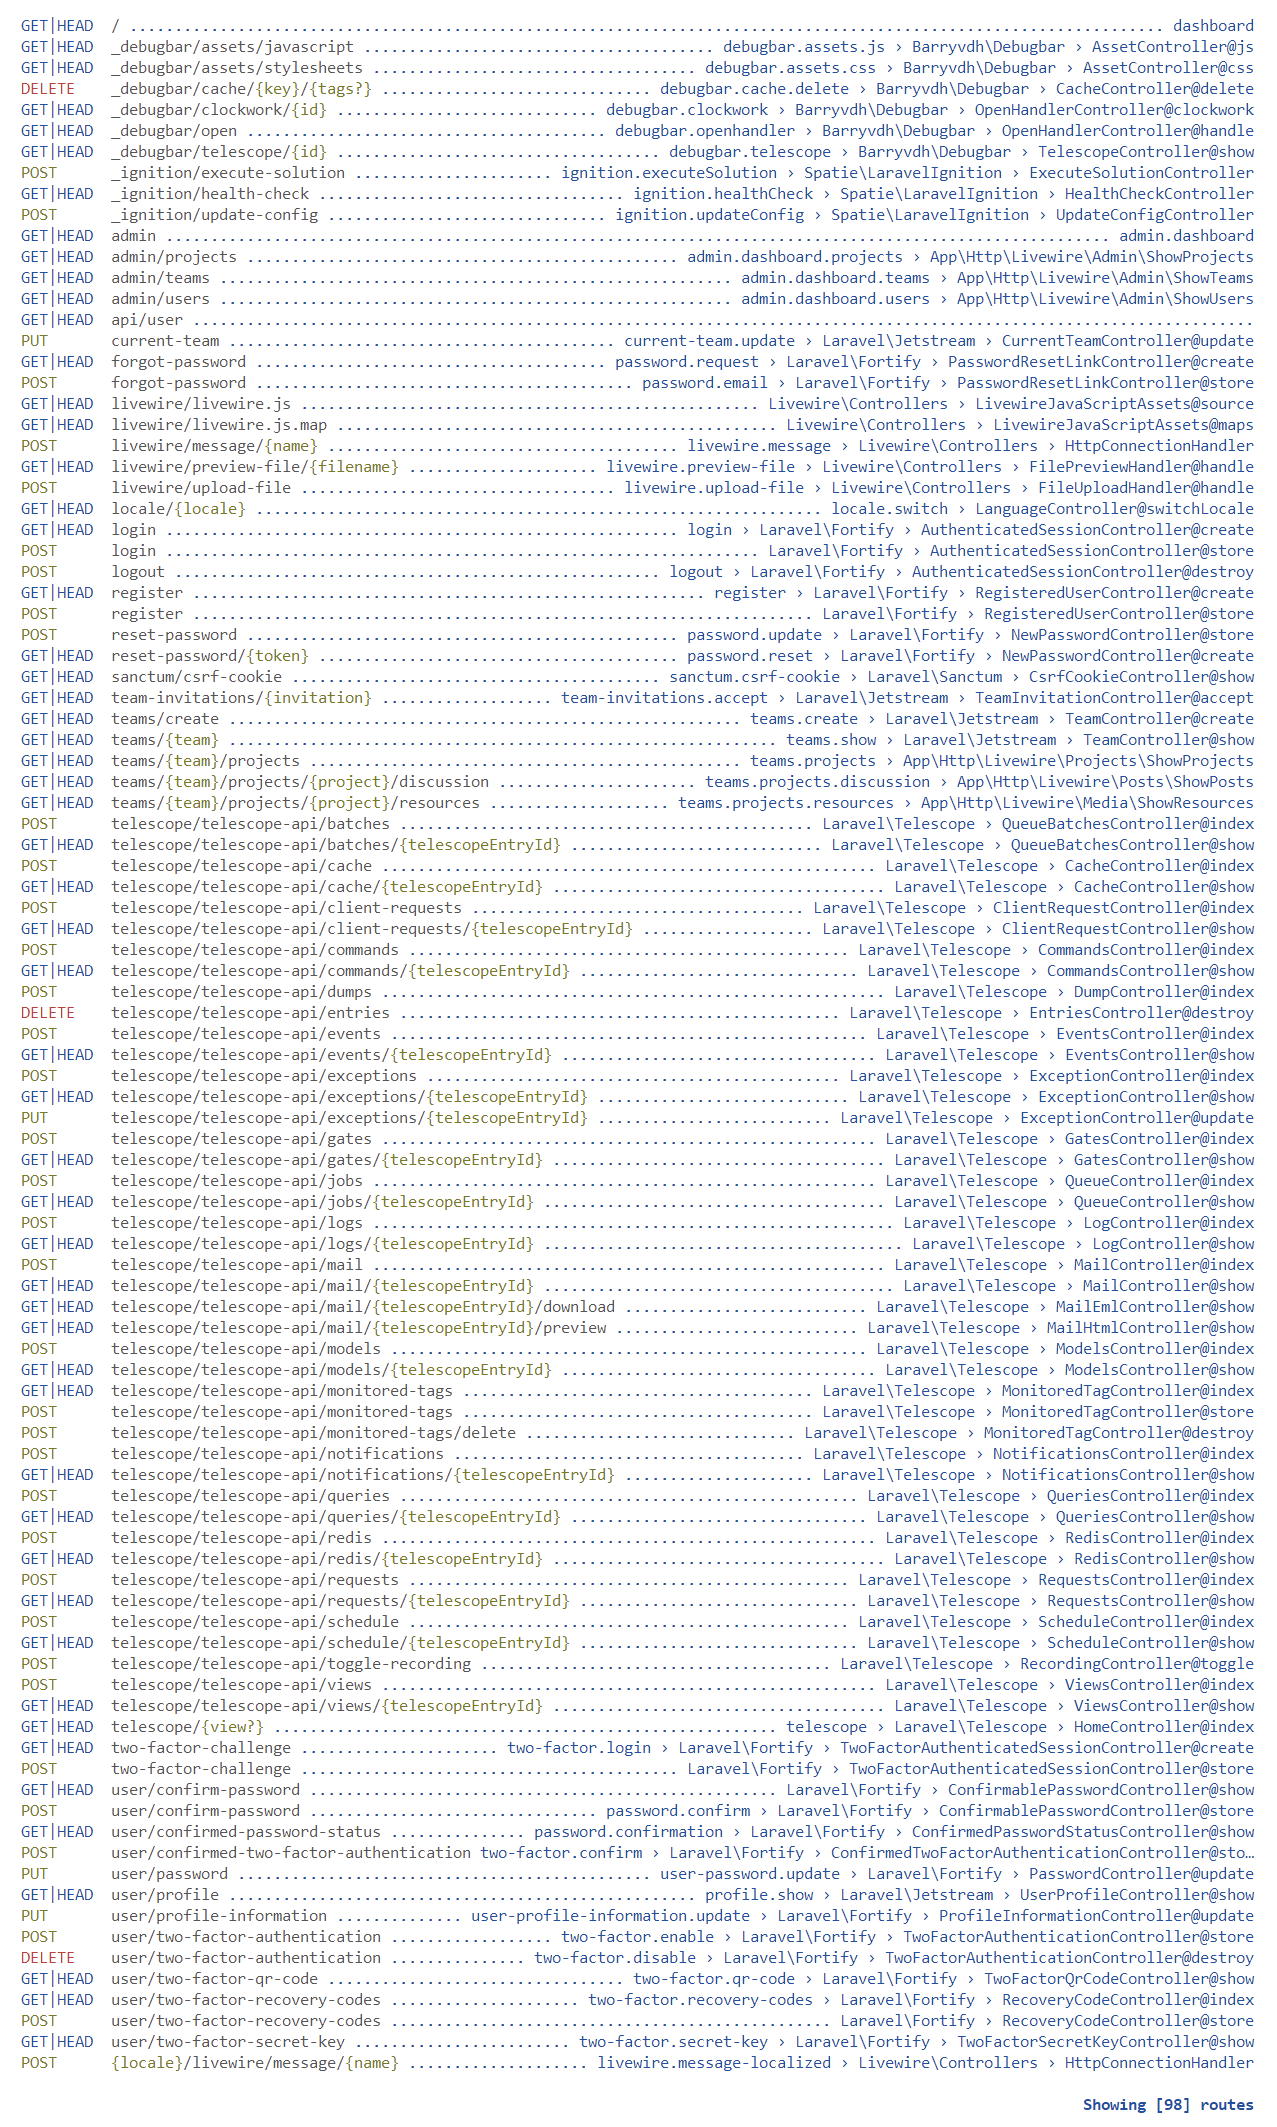
\includegraphics[width=0.9\linewidth,clip=]{assets/routes.png}
	\centering
	\caption{Izlist svih ruta definiranih u aplikaciji pomoću  Artisan naredbe \texttt{route:list}}
	\label{fig:routes}
\end{figure}

\subsection{Middleware}
\textit{Middleware}, srednji sloj Laravel web aplikacije, mehanizam je za pregled, filtriranje i kontrolu korisničkih HTTP zahtjeva koji dolaze aplikaciji. Nekoliko \textit{middlewarea} zadano je uključeno u razvojni okvir Laravel, uključujući onaj za autentikaciju i CSRF zaštitu. Sve \textit{middleware} klase nalaze se u direktoriju \texttt{app/Http/Middleware} te se novi \textit{middleware} može stvoriti Artisan naredbom \texttt{make:middleware}~\cite{middleware}.

U ispisu~\ref{configureLocaleMiddleware} prikazan je \texttt{ConfigureLocale} \textit{middleware} napisan za potrebe implementacije lokalizacije.

\begin{lstlisting}[caption={\textit{Middleware} \texttt{ConfigureLocale}}, label=configureLocaleMiddleware]
<?php

namespace App\Http\Middleware;

use Closure;
use Illuminate\Http\Request;
use Illuminate\Support\Facades\App;
use Illuminate\Support\Facades\Session;
use Symfony\Component\HttpFoundation\Response;

class ConfigureLocale
{
    /**
     * Handle an incoming request.
     *
     * @param  \Closure(\Illuminate\Http\Request): (\Symfony\Component\HttpFoundation\Response)  $next
     */
    public function handle(Request $request, Closure $next): Response
    {
        if ($request->has('locale')) {
            $locale = $request->get('locale');
            Session::put('locale', $locale);
        }

        if (Session::has('locale') && array_key_exists(Session::get('locale'), config('locales'))) {
            App::setLocale(Session::get('locale'));
        } else {
            App::setLocale(config('app.fallback_locale'));
        }

        return $next($request);
    }
}

\end{lstlisting}

Pojedini \textit{middleware} treba se registrirati u aplikaciji - ako se želi da je aktivan globalno dodaje ga se među vrijednosti podatkovnog člana \texttt{\$middleware} klase \\ \texttt{app/Http/Kernel.php}, a ako se želi da djeluje na pojedinoj ruti na nju ga se dodaje pomoću metode \texttt{middleware}. Radi jednostavnosti i praktičnosti, unutar klase \\ \texttt{app/Http/Kernel.php} u podatkovnom članu \texttt{\$middlewareAliases} pojedinom \textit{middlewareu} se može nadjenuti \textit{alias} ime~\cite{middleware} (pogledati ispis~\ref{middlewareAliases}).

\begin{lstlisting}[caption={Definiranje \textit{middleware} \textit{aliasa}}, label=middlewareAliases]
    /**
     * The application's middleware aliases.
     *
     * Aliases may be used to conveniently assign middleware to routes and groups.
     *
     * @var array<string, class-string|string>
     */
    protected $middlewareAliases = [
        'auth' => \App\Http\Middleware\Authenticate::class,
        'auth.basic' => \Illuminate\Auth\Middleware\AuthenticateWithBasicAuth::class,
        'auth.session' => \Illuminate\Session\Middleware\AuthenticateSession::class,
        'cache.headers' => \Illuminate\Http\Middleware\SetCacheHeaders::class,
        'can' => \Illuminate\Auth\Middleware\Authorize::class,
        'guest' => \App\Http\Middleware\RedirectIfAuthenticated::class,
        'password.confirm' => \Illuminate\Auth\Middleware\RequirePassword::class,
        'signed' => \App\Http\Middleware\ValidateSignature::class,
        'throttle' => \Illuminate\Routing\Middleware\ThrottleRequests::class,
        'verified' => \Illuminate\Auth\Middleware\EnsureEmailIsVerified::class,
        'locale' => \App\Http\Middleware\ConfigureLocale::class,
    ];
\end{lstlisting}

Različite \textit{middleware} klase može se međusobno grupirati pod istim ključem (engl. \textit{key}) u prethodno navedenoj \texttt{Kernel} klasi  koristeći podatkovni član \texttt{\$middlewareGroups}~\cite{middleware} (pogledati ispis~\ref{middlewareGroups}).


\begin{lstlisting}[caption={Definiranje \textit{middleware} grupa}, label=middlewareGroups]
    /**
     * The application's route middleware groups.
     *
     * @var array<string, array<int, class-string|string>>
     */
    protected $middlewareGroups = [
        'web' => [
            \App\Http\Middleware\EncryptCookies::class,
            \Illuminate\Cookie\Middleware\AddQueuedCookiesToResponse::class,
            \Illuminate\Session\Middleware\StartSession::class,
            \App\Http\Middleware\ConfigureLocale::class,
            \Illuminate\View\Middleware\ShareErrorsFromSession::class,
            \App\Http\Middleware\VerifyCsrfToken::class,
            \Illuminate\Routing\Middleware\SubstituteBindings::class,
        ],

        'api' => [
            // \Laravel\Sanctum\Http\Middleware\EnsureFrontendRequestsAreStateful::class,
            \Illuminate\Routing\Middleware\ThrottleRequests::class.':api',
            \Illuminate\Routing\Middleware\SubstituteBindings::class,
        ],
    ];
\end{lstlisting}

\subsection{Autentikacija}

\subsection{Autorizacija}

\subsubsection{Politike (engl. \textit{policies})}

\subsubsection{Vrata (engl. \textit{gates})}

\subsection{Livewire komponente}

\subsubsection{Akcije}

\subsubsection{Događaji}

\subsection{Pohrana datoteka}

\subsubsection{MinIO - AWS S3 kompatibilan servis za pohranu}

\subsection{Spatie Laravel Media Library paket}

\subsection{Lokalizacija}
\label{subsection:localization}

\subsection{Testiranje i kvaliteta k\^oda}

\subsubsection{Korišteni alati}
\textbf{Laravel Debug Bar}, \textbf{Laravel Telescope}, \textbf{Laravel Pint}, pretpregled elektroničke pošte - \textbf{MailHog}

\subsubsection{Pisanje i pokretanje testova}

\subsection{Otvoreni k\^od i doprinos zajednice na projektima Laravel ekosustava}
